\chapter{Olhó-passarinho}\label{chap:chap4}

Neste capitulo será abordado a ferramenta desenvolvida com a descrição da arquitetura sistema implementado, do processamento da informação espaço-temporal e da sua integração com a informação visual de modo a aplicar a tarefa de \textit{clustering}. Por fim será apresentado a visualização dos resultados ilustrativos e consequentemente a sua discussão. 

\section{Arquitetura do Sistema}

A arquitetura do sistema desenvolvido é apresentado na figura~\ref{fig:archsys}. Este apresenta uma divisão entre os serviços externos e o modelo desenvolvido. Este modelo foi desenhado de modo a que existisse uma separação entre o tratamento de toda a parte de processamento dos dados e a visualização, existindo assim um \textit{back-end} com todos os ficheiros e módulos desenvolvidos e um \textit{front-end} que representa a aplicação web para visualização dos resultados. No \textit{back-end} existe também uma divisão entre dois módulos fundamentais, o módulo de processamento da informação visual, responsável por tratar a informação das imagens como descrito no Capítulo~\ref{chap:chap3}, de modo a que essa informação possa ser utilizada pelo módulo responsável pelo processo de \textit{Data Mining} já desenvolvido no TweeProfiles~\cite{Cunha2013}. 

Os serviços externos correspondem à base de dados Mongodb para a recolha dos tweets e os serviços Twitter e Instagram para a recolha das imagens através do URL. No caso do modelo desenvolvido, a parte de \textit{back-end} possuí os ficheiros JSON com os dados e as imagens necessárias, tanto para o módulo de processamento da informação visual como para a extração e processamento do dados espaço-temporais, explicados na próxima secção~\ref{sec:infoesptmp}. Os dados processados no módulo da informação visual e os dados espaço-temporal extraídos dos tweets são assim utilizados no processo de \textit{Data Mining}, onde é aplicada a tarefa de \textit{clustering} como explicado na secção~\ref{sec:finalclustering} apresentada mais adiante. De este processo resultam os \textit{clusters} calculados através de vários parâmetros, sendo estas informações armazenadas em ficheiros. Por fim, foi utilizada a \textit{microframework} Flask para desenvolvimento de aplicações web em Python, que permitiu o desenvolvimento da aplicação Olhó-passarinho para visualização dos resultados. 

\begin{figure}[h]
\centering
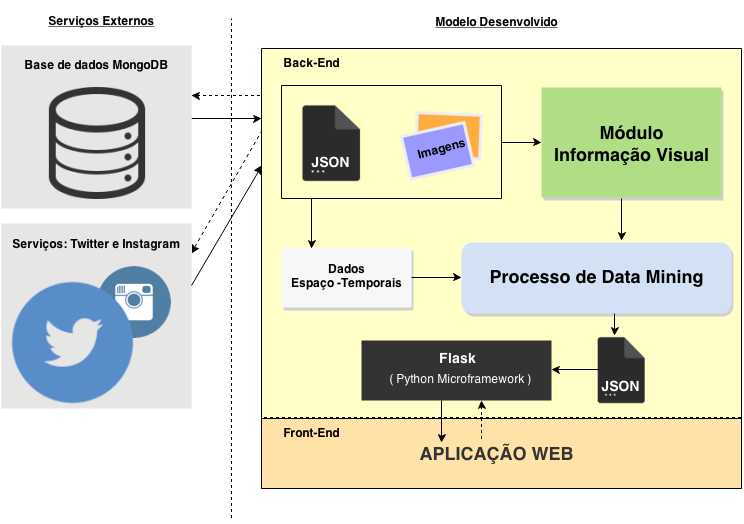
\includegraphics[width=1.0\linewidth]{./figures/arquitetura_sistema}
\caption{Arquitetura do sistema completo}
\label{fig:archsys}
\end{figure}


\section{Informação Espaço-Temporal} \label{sec:infoesptmp}

Uma das características principais tanto do TweeProfiles como do Olhó-paddarinho e é integração das dimensões espaço-temporais com o conteúdo. Tal como no foi efetuado no TweeProfiles, também aqui foi utilizado estas dimensões, tendo sido então recolhido a informação de tempo e espaço dos tweets para o cálculo das respetivas matrizes de distância entre tweets.

Em primeiro lugar foi recolhida a informação espacial. Neste caso os dados possuem a informação de latitude e longitude do ponto onde foi enviado o tweet. Para calcular a distância entre tweets utilizou-se a função distância Haversine abordada no capítulo~\ref{chap:estarte} na subsecção~\ref{subsubsec:space}. Neste caso foi calculada a distância em quilómetros, tendo sido considerado o valor do raio da Terra igual a 6371 Km.

Posteriormente foi então recolhida a informação temporal dos tweets. Esta informação apresenta-se no seguinte formato:

\vspace{2mm}
Tue Jun 18 17:02:09 +0000 2013
\vspace{2mm}

Para o cálculo da distância entre datas foi utilizada a função distância euclidiana, que se pode resumir ao módulo da diferença entre o tempo de dois tweets, como pode ser visto no capítulo~\ref{chap:estarte} na subsecção~\ref{subsubsec: time}. Utilizando as bibliotecas \textit{datetime} e \textit{dateutil} este cálculo é direto sem necessitar ser realizada uma conversão do formato da data.

%\textbf{Nota:} Devo colocar mais informação estatística sobre os dados?

\section{Clustering da Informação Visual, Espacial e Temporal} \label{sec:finalclustering}

A tarefa de \textit{clustering} é o passo final para a obtenção dos resultados finais. Este é o processo que engloba os dados resultantes de todo o processamento da informação tratada e discutida anteriormente.

Para a tarefa de \textit{clustering} optou-se pela utilização do algoritmo implementado no TweeProfiles~\cite{Cunha2013}, o DBSCAN. Este apresenta algumas vantagens na utilização de dados recolhidos de redes sociais, pois este não necessita de uma predefinição do número de \textit{clusters} que se pretende obter, sendo o número de \textit{clusters} é definido através da distribuição em densidade dos objetos, como referido no capítulo~\ref{chap:estarte} na subsecção~\ref{subsec:dbscan}.

Mas antes de fornecer os dados, neste caso as matrizes já calculadas com as distâncias entre tweets para as dimensões temporal, espacial e de conteúdo visual, foi necessário recorrer a sua normalização de modo a que fosse possível a combinação entre as várias matrizes. Foi então utilizada a normalização através da média e do desvio padrão.
%colocar formula de normalização e confirmar se foi esta a normalização utilizada

Após a normalização, realizou-se a combinação entre as matrizes, com atribuição de vários pesos a cada matriz, de forma a que a soma dos diferentes pesos fosse igual a 1. Inicialmente, a distribuição dos pesos foi feita com passos de 0.25 pontos, isto é, os valores de cada matriz podiam assumir os pesos: 0, 0.25, 0.5, 0.75 e 1. Isto permitiu uma fácil divisão dos pesos, mas não permitia atribuir pesos iguais às três matrizes, pelo número de matrizes ser ímpar. Assim, optou-se por dividir os pesos em fator de 0.333, em que os valores de cada matriz podem assumir os pesos: 0, 0.333, 0.666, 1. Isto faz que a soma dos pesos posa não dar exatamente 1, mas sim 0.999. Por outro lado, isto possibilitou atribuir o mesmo peso às três matrizes diferentes de cada subconjunto.

%A distribuição dos pesos foi feita com passos de 0.25 pontos, isto é, os valores de cada matriz podem assumir os pesos: 0, 0.25, 0.5, 0.75 e 1, sendo que, como referido, a soma dos pesos tem necessariamente de ser igual a 1

A tabela~\ref{tab:pesos} apresenta as diferentes combinações possíveis de pesos para as diferentes dimensões

\begin{table}[h]
\centering
\begin{tabular}{|c|c|c|c|}
\hline
\textbf{Combinação} & \textbf{Visual} & \textbf{Espacial} & \textbf{Temporal} \\ \hline
1 & 1.000 & 0.000 & 0.000 \\ \hline
2 & 0.666 & 0.333 & 0.000 \\ \hline
3 & 0.666 & 0.000 & 0.333 \\ \hline
4 & 0.333 & 0.333 & 0.333 \\ \hline
5 & 0.000 & 1.000 & 0.000 \\ \hline
6 & 0.333 & 0.666 & 0.000 \\ \hline
7 & 0.000 & 0.666 & 0.333 \\ \hline
8 & 0.000 & 0.000 & 1.000 \\ \hline
9 & 0.333 & 0.000 & 0.666 \\ \hline
10 & 0.000 & 0.333 & 0.666 \\ \hline
\end{tabular}
\vspace{2 mm}
\caption{Tabela com as possiveis distribuições de pesos entre as várias dimensões}
\label{tab:pesos}
\end{table}

\section{Visualização}

A aplicação web desenvolvida é a responsável pela visualização dos resultados obtidos pela tarefa de \textit{clustering}. Esta apresenta três secções principais de visualização dos \textit{clusters} pelas diferentes dimensões utilizadas. 

O primeiro é um mapa, onde são apresentados a distribuição dos tweets, como pode ser visto na figura~\ref{fig:map1} e a respetiva distribuição dos \textit{clusters} geograficamente. Este foi desenvolvido recorrendo à API Javascript do Google Maps v3~\cite{googlemapsapi} disponibilizada pela própria Google, sendo toda ela controlada através da linguagem de programação Javascript. Esta permite utilizar um mapa e controlar de modo a adicionar componentes a esse mapa. Os tweets foram assim representados por pequenos círculos azuis, e os \textit{clusters} como círculos vermelhos com transparência. 

\begin{figure}[h]
\centering
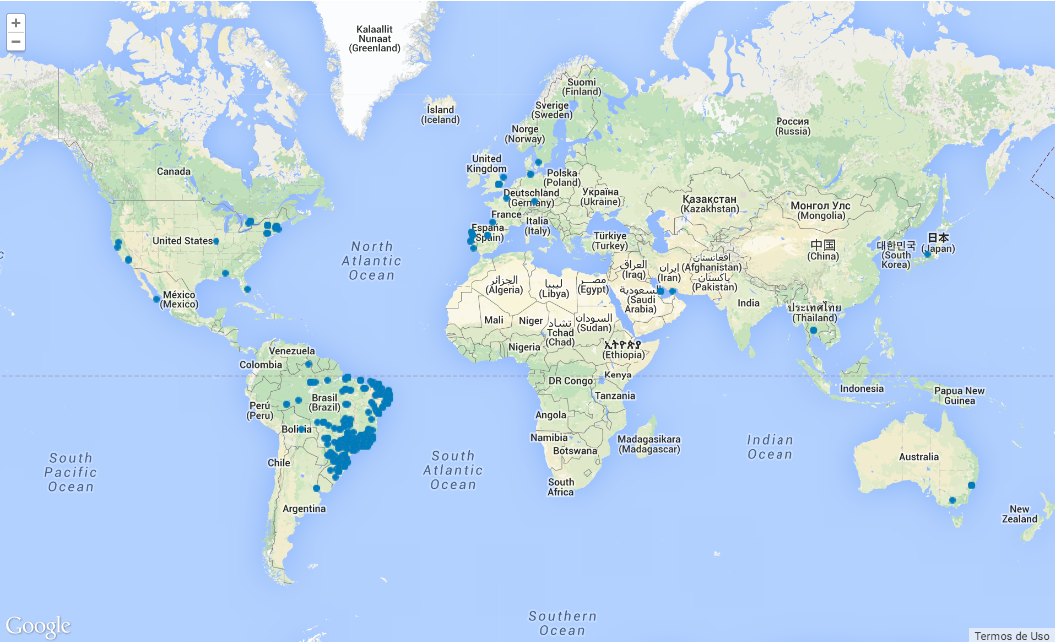
\includegraphics[width=1.0\linewidth]{./figures/olhopassarinho/map1.png}
\caption{Distribuição de tweets na dimensão espacial}
\label{fig:map1}
\end{figure}

A segunda secção é responsável pela representação da distribuição dos \textit{clusters} na dimensão temporal e foi utilizado a ferramenta Google Charts, mais especificamente a API Timeline~\cite{googletimeline}. Esta, tal como a API do Google Maps, também é desenvolvida em javascript, e permite reproduzir um gráfico com barras de duração temporal, como podemos ver na figura~\ref{fig:timeex}. 

\begin{figure}[h]
\centering
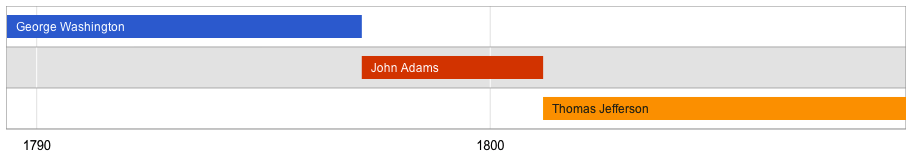
\includegraphics[width=1.0\linewidth]{./figures/olhopassarinho/time_example.png}
\caption{Exemplo ilustrativo da ferramenta Timeline. \textit{Retirada de}~\cite{googletimeline}}
\label{fig:timeex}
\end{figure}

Por último, a secção de visualização de imagens que pertencem a um \textit{cluster}. Nesta é apresentado uma matriz com nove imagens presentes nos \textit{clusters} escolhidas aleatoriamente, havendo ainda a possibilidade de ir modificando as imagens visíveis. É possível também clicar numa das imagens e visualizar a imagem numa dimensão maior e ver a informação relativa à imagem como o utilizador que fez a partilha e o texto partilhado em conjunto. Para além disto, é possível aceder ao tweet original através de um botão com essa indicação. Esta secção também indica o nome do \textit{cluster} e a informação temporal em texto do mesmo.

A aplicação apresenta também os controlos para escolher o subconjunto que se pretende visualizar, e controlos para definir o peso que se pretende atribuir a cada dimensão.

\section{Resultados Ilustrativos}

Nesta secção serão apresentados alguns resultados ilustrativos visíveis através ferramenta Olhó-passarinho. Neste relatório não é possível apresentar todos os resultados devido ao número de diferentes possíveis combinações. 

A Figura~\ref{fig:map3} mostra um exemplo da visualização da distribuição dos \textit{clusters} no espaço geográfico. Este exemplo é relativo a uma divisão igual dos pesos entre as três dimensões, espacial, temporal e as fotografias, tendo cada uma um peso de 33.33\% nos resultados dos \textit{clusters}.

\begin{figure}[h]
\centering
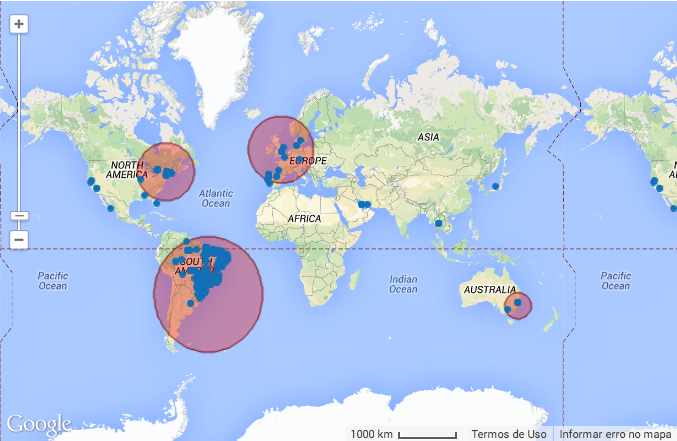
\includegraphics[width=0.6\linewidth]{./figures/olhopassarinho/map3}
\caption{Exemplo ilustrativo da visualização da distribui espacial dos \textit{clusters} para o caso em que a distribuição dos pesos entre as três dimensões é igual}
\label{fig:map3}
\end{figure}

A dimensão dos círculos que representam os \textit{clusters} é proporcional ao número de tweets presentes nesse mesmo \textit{clusters} isto é, quanto maior o número de tweets maior é a respetiva circunferência.

Já Figura~\ref{fig:time2} apresenta a distribuição dos cinco diferentes \textit{clusters} da mesma situação anterior, sendo possível visualizar a existência de \textit{clusters} com uma margem de maior duração, enquanto outros como o caso do \textit{Clusters 3} que apresenta uma duração de menos de 4 horas. A distribuição no tempo do conjunto de tweets utilizados para este exemplo, como podemos ver na Figura~\ref{fig:time2}, é de aproximadamente 24 horas, em que teve início no dia 17 de Junho de 2013 e terminou no dia 18 de Junho de 2013.

\begin{figure}[h]
\centering
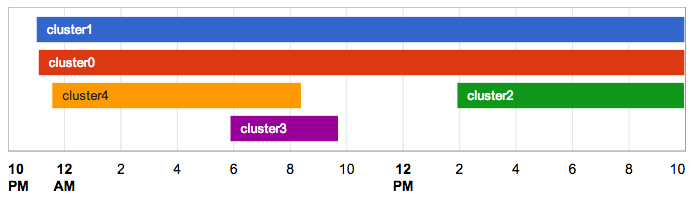
\includegraphics[width=0.7\linewidth]{./figures/olhopassarinho/time2}
\caption{Exemplo ilustrativo da visualização da distribui temporal dos \textit{clusters} para o caso em que a distribuição dos pesos entre as três dimensões é igual}
\label{fig:time2}
\end{figure}

A Figura~\ref{fig:exemplocomp} traz-nos uma perspetiva global da aplicação web, mostrando mais detalhe sobre um dos \textit{clusters}, neste caso o \textit{Cluster 2}. Na Figura~\ref{fig:exemplocomp} é possível a visualização de nove imagens aleatórias do \textit{Cluster 2}. Já no caso da Figura~\ref{fig:exemplocomp2}, é apresentado a visualização mais pormenorizada de uma das imagens, com a indicação do nome do autor do tweet e a mensagem associada à imagem partilhada pelo mesmo. Também é possível aceder ao tweet original.

\begin{figure}[h]
\centering
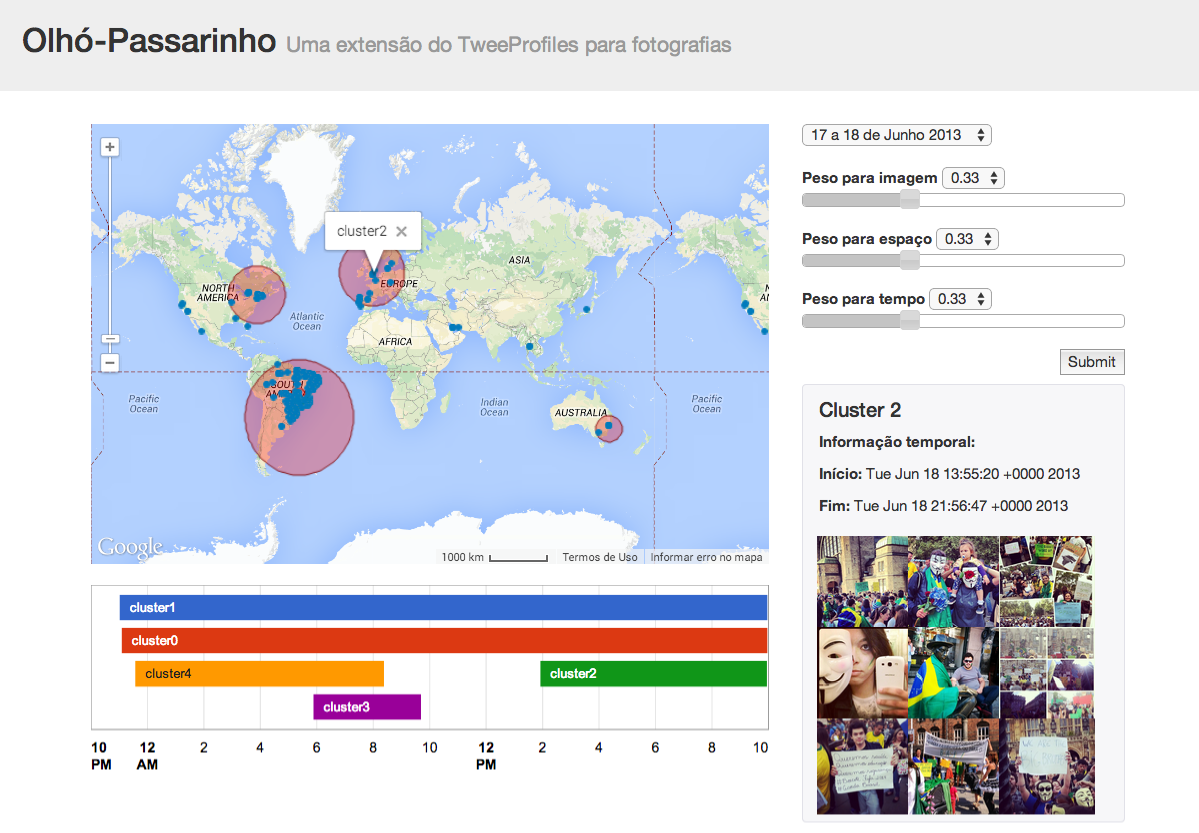
\includegraphics[width=0.8\linewidth]{./figures/olhopassarinho/exemplo_comp}
\caption{Exemplo ilustrativo da visualização completa da aplicação web com a visualização pelas várias dimensões}
\label{fig:exemplocomp}
\end{figure}

\begin{figure}[h]
\centering
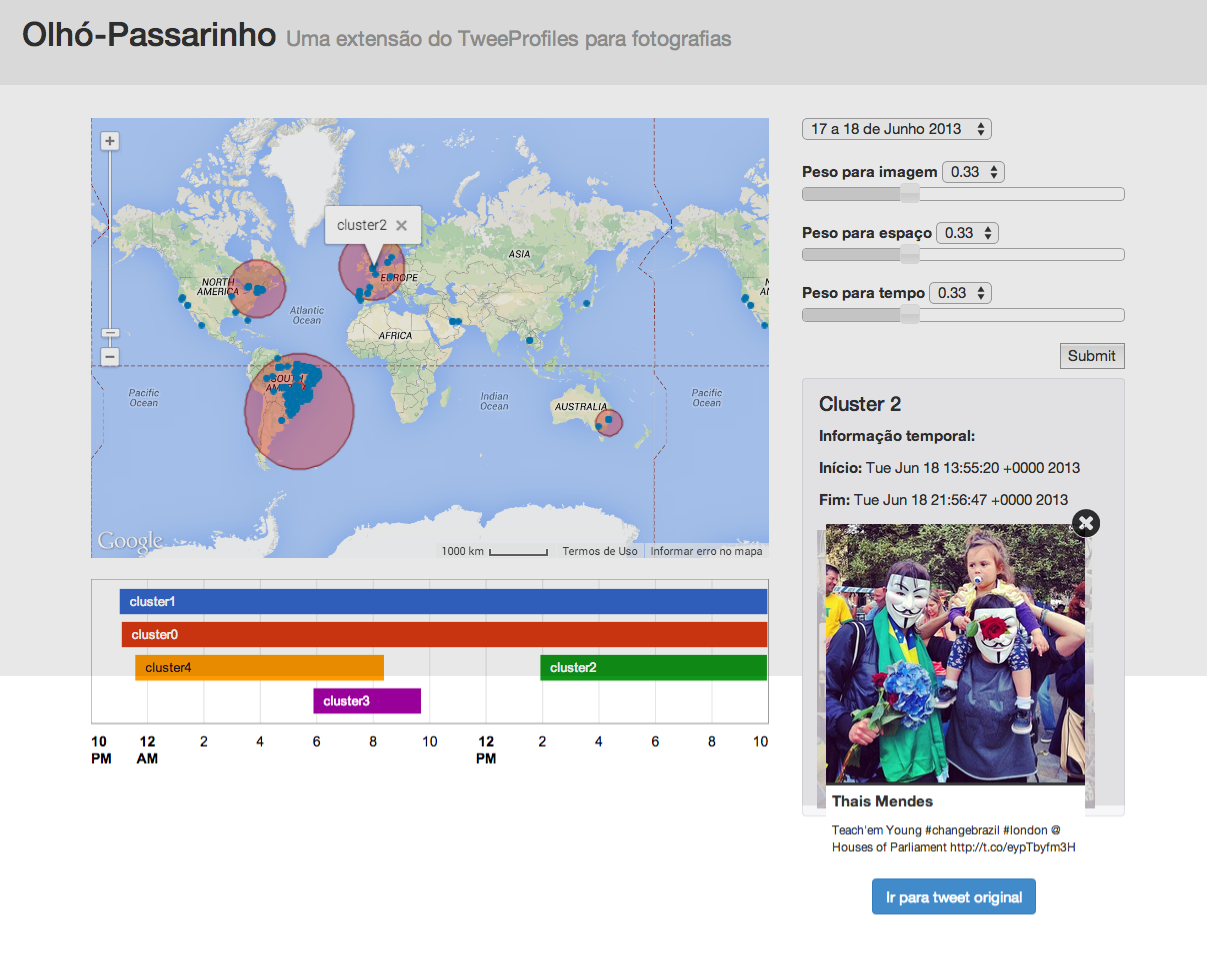
\includegraphics[width=0.8\linewidth]{./figures/olhopassarinho/exemplo_comp2}
\caption{Exemplo ilustrativo da visualização completa da aplicação web com a visualização mais detalhada de uma das imagens}
\label{fig:exemplocomp2}
\end{figure}

\begin{figure}[h]
\centering
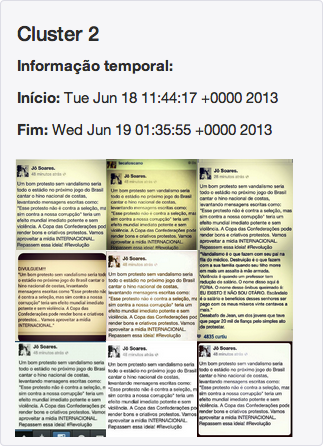
\includegraphics[width=0.8\linewidth]{./figures/olhopassarinho/im1}
\caption{Exemplo ilustrativo da visualização de um conjunto de imagens pertencentes a um \textit{Cluster} e em que foi atribuído o peso total apenas à dimensão do conteúdo visual}
\label{fig:ims}
\end{figure}

É interessante salientar que no exemplo ilustrado na Figura~\ref{fig:exemplocomp} existe uma semelhança geral entre as nove imagens, sendo isto possível, devido a combinação das três dimensões, tendo sido agrupado tweets com semelhança nas imagens, mas também no espaço e tempo.


Outro exemplo interessante, é quando a atribuição do peso de 100\% apenas para a dimensão do conteúdo visual. A Figura~\ref{fig:ims} demonstra um exemplo desses, e como é visível, o \textit{cluster} possuí pelo menos nove imagens muito semelhantes, que apesar de não fazerem parte de um evento que inclua pessoas, este permitiu encontrar a partilha de várias partilhas de um mesmo texto por várias pessoas através de uma imagem. Este resultado também vem demonstrar que o modelo responsável pela extração da informação visual apresentou um bom desempenho, tal como era o esperado.

